\documentclass{article}
\usepackage{graphicx}
\usepackage{amsmath}
\usepackage{float}
\usepackage{amsfonts}
\usepackage{listings}
\usepackage{xcolor}
\usepackage[utf8]{inputenc}
\usepackage{hyperref}
\usepackage{fancybox}
\usepackage[labelfont=bf, font=small]{caption}  % Pour personnaliser le titre de la figure


\lstset{
  language=R,
  basicstyle=\ttfamily\small,
  numbers=left,               % Numérotation des lignes
  numberstyle=\tiny\color{gray}, % Style de la numérotation
  keywordstyle=\color{blue},  % Couleur des mots-clés
  commentstyle=\color{green}, % Couleur des commentaires
  stringstyle=\color{red},    % Couleur des chaînes de caractères
  breaklines=true,            % Coupe les lignes trop longues
  frame=single,               % Encadre le code
}


\title{TP1 TID}
\author{SCAIA Matteo, MARIAC Damien}
\date{\today} 

\begin{document}

\maketitle

\begin{figure}[h] 
    \centering
    
\includegraphics[width=0.5\textwidth]{ssd_logo.png} 
\end{figure}

\begin{figure}[h] 
    \centering
    
\includegraphics[width=0.5\textwidth]{logo_um_2022_rouge_RVB.png} 
\end{figure}

\newpage

\tableofcontents

\newpage

\section{Exercice 1}
On considère le tableau ci-dessous, répartissant la population active occupée selon l'âge ($A$), le sexe ($S$) et la
catégorie socioprofessionnelle ($C$) (source: INSEE, enquête emploi 2016).
\begin{figure}[ht]
  \centering
  \setlength{\fboxsep}{0pt}  % Pour que l'image soit bien ajustée dans le cadre
  \setlength{\fboxrule}{1pt}  % Épaisseur du cadre
  \fbox{%
    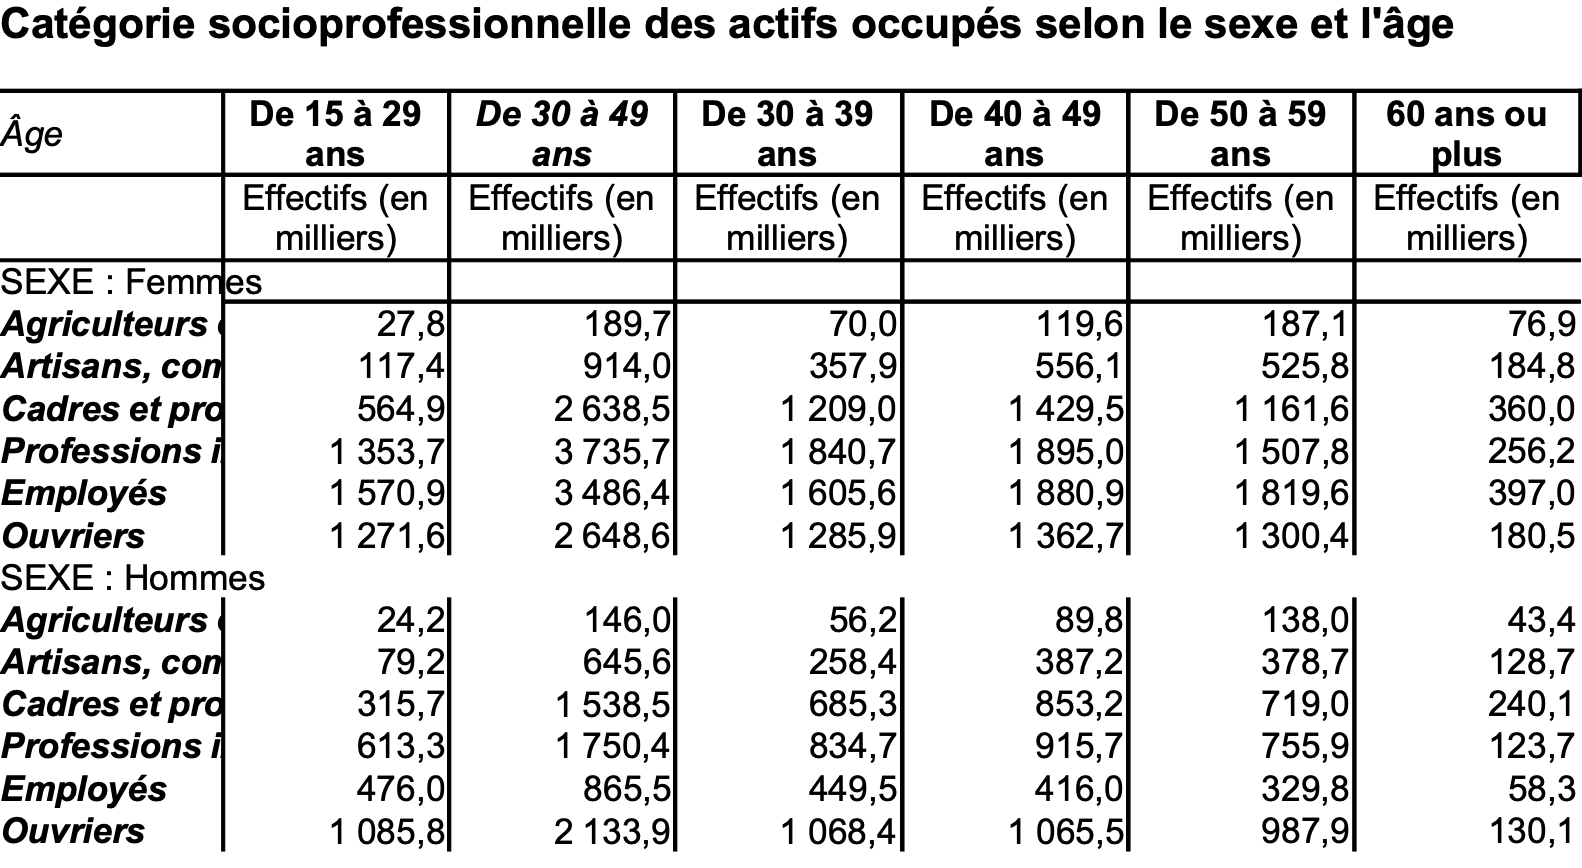
\includegraphics[width=0.7\textwidth]{CE.png}
  }
  \caption{Tableau répartissant la population active occupée selon des catégories }
\end{figure}
\subsection{Modélisation et variable}
\label{1.1}
Tout d'abord de manière intuitive, nous avons envie de modéliser la variable
socioprofessionnelle avec les deux autres. Cependant, nous devons
le montrer de manière formelle. Grâce au code fourni dans la partie \ref{sec : Annexe},
nous calculons l'information mutuelle de chacune des variables.\\\\
Premièrement, nous calculons l'entropie de chacune de ces variables.\\
Pour la variable $A$, nous avons le tableau suivant (en fréquence). 
\begin{table}[ht]
  \centering
  \begin{tabular}{|l|l|l|l|l|l|l|}
    \hline
    & 15-29 ans  & 30-39 ans  & 40-49 ans  & 50-59 ans  & 60+ ans \\ \hline
    Age & 0.1866 & 0.2419 & 0.2730 & 0.2441 & 0.0542 \\ \hline
  \end{tabular}
  \caption{Distribution par âge ($A$)}
\end{table}
\\Nous pouvons calculer l'entropie de $A$.\\
\[
H(A) = -\sum_{n = 1}^{6}p_i\log_2(p_i)=2,1833
\]
De même manière, nous calculons l'entropie de $C$ et $S$.\\
\begin{table}[H]
  \centering
  \begin{tabular}{|l|l|l|}
  \hline
             & Femme  & Homme  \\ \hline
  Proportion & 0,6589 & 0,3411 \\ \hline
  \end{tabular}
  \caption{Distribution par sexe ($S$)}
\end{table}

\begin{table}[H]
  \centering
  \begin{tabular}{|l|l|l|l|l|l|l|}
  \hline
             & Agriculteur & Artisans & Cadres & Profession In & Employes & Ouvrier \\ \hline
  Proportion & 0,0207      & 0,0740   & 0,1875 & 0,2512        & 0,2240   & 0,2423  \\ \hline
  \end{tabular}
  \caption{Distribution par catégorie socioprofessionnelle ($C$)}
  \end{table}


Nous obtenons.
\[
H(S) = 0,9258  \hspace{2 cm} H(C)= 2,3266
\]
A présent, nous devons calculer les valeurs suivantes : $H(A,S)$, $H(A,C)$ et $H(S,C)$.\\
\begin{table}[H]
  \centering
  \begin{tabular}{|l|l|l|l|l|l|}
  \hline
        & 15-29 ans & 30-39 ans & 40-49 ans & 50-59 ans & 60+    \\ \hline
  Femme & 0,1220    & 0,1584    & 0,1803    & 0,1618    & 0,0362 \\ \hline
  Homme & 0,0645    & 0,0834    & 0,0927    & 0,0823    & 0,1802 \\ \hline
  \end{tabular}
  \caption{Distribution jointe sexe ($S$) et âge ($A$)}
  \end{table}

  \begin{table}[H]
    \centering
    \begin{tabular}{|l|l|l|l|l|l|}
    \hline
                   & 15-29 ans & 30-39 ans & 40-49 ans & 50-59 ans & 60+    \\ \hline
    Agriculteur    & 0,0013    & 0,0031    & 0,0052    & 0,0081    & 0,0030 \\ \hline
    Artisans       & 0,0049    & 0,0153    & 0,0234    & 0,0225    & 0,0080 \\ \hline
    Cadres         & 0,0219    & 0,0471    & 0,0568    & 0,0468    & 0,0149 \\ \hline
    Professions In & 0,0489    & 0,0665    & 0,0699    & 0,0563    & 0,0094 \\ \hline
    Employes       & 0,0509    & 0,0511    & 0,0571    & 0,0535    & 0,0113 \\ \hline
    Ouvrier        & 0,0586    & 0,0586    & 0,0604    & 0,0569    & 0,0077 \\ \hline
    \end{tabular}
    \caption{Distribution jointe ($C$) et âge ($A$)}
    
  \end{table}

\begin{table}[H]
  \centering
  \begin{tabular}{|l|l|l|l|l|l|l|}
  \hline
         & Agriculteur & Artisans & Cadres & Profession IN & Employes & Ouvrier \\ \hline
    Femmes & 0.0119      & 0.0433   & 0,1175 & 0.1705        & 0.1810   & 0.1344  \\ \hline
    Homme  & 0.0087      & 0.0307   & 0,0700 & 0.0807        & 0.0430   & 0.1079  \\ \hline
    \end{tabular}
    \caption{Distribution jointe ($C$) et ($S$)}
\end{table}
Nous obtenons les valeurs suivantes.
\[
H(A,S)=3,1092 \hspace{1 cm} H(A,C)= 4,4817 \hspace{1cm} H(C,S)=3,2242
\]
De plus, nous obtenons pour $H(A,S,C)$ la valeur suivante.
\[
  H(A,C,S) = -\sum_{n = 1}^{72}p_i\log_2(p_i)=5,3778
\]
Nous pouvons calculer les informations mutuelles.
\[
I(C,(AS))=H(C)+H(A,S)-H(A,S,C) = 0,0580 \\
\]
\[
I(A,(SC))= 0,029803
\]
\[
I(S,(CA))=0,029813
\]
Cherchons le rapport entre l'information mutuelle et la variable conditionnée le plus élevé.
\[
R_1 = \frac{I(C,(AS))}{H(A,C)}=0,0187
\]
\[
R_2 = \frac{I(A,(SC)))}{H(S,C)}=0,0092
\]
\[
R_3 = \frac{I(S,(CA)))}{H(A,C)}=0,0066
\]
Le rapport $R_1$ est le plus élevé. Donc c'est la variable $C$ modélisé par les deux autres ($A$ et $S$) qui nous donne le plus d'information.
\subsection{Arbre de segmentation binaire}
Grâce à la partie \ref{1.1}, nous pouvons calculer les informations mutuelles suivantes.
\[
I(A,S) = H(A) + H(S) - H(A,S) = 5,1104*10^{-5}
\]
\[
I(A,C) = 0,02830
\]
\[
I(S,C)= 0,02831
\]
Faisons, la somme de ses informations mutuelles avec chacune des deux autres.
\[
\bar{I_A} = I(A,S) + I(A,C) = 0,02835
\]
\[
\bar{I_S}= 0,02836 
\]
\[
\bar{I_C} = 0,0566
\]
Nous avons donc $\bar{I_C}$ qui est le plus élevé. Ainsi, l'arbre de segmentation commencera avec la variable $C$.




\newpage
\section{Exercice 2}
\subsection{Recodages}

\subsubsection{Recodage en 2 variables}

En agrégeant seulement les classes contigues, nous avons 4 possibilités de regroupement binaire de 
X.
\\

\[
Z1 =\{ \{0 \% \} , \{0 - 0.5 \% ,0.5-1 \% ,1-3 \% ,>3 \% \} \}  
\]
\[
Z1 =\{ \{0 \% , 0 - 0.5 \%  \} , \{0.5-1 \% ,1-3 \% ,>3 \% \} \}
\]
\[
Z1 =\{ \{0 \%, 0 - 0.5 \% ,0.5-1 \%  \} , \{1-3 \% ,>3 \% \} \}
\]
\[
Z1 =\{ \{0 \% , 0 - 0.5 \% ,0.5-1 \% ,1-3 \% \} , \{>3 \% \} \}
\]
\\

L'entropie de chacun de ses recodages se calcule numeriquement et donne :

\[
H(Z1) = -(29/72*log2(29/72)+43/72*log2(43/72)) = 0.973
\]
\[
H(Z2) = -(29/72*log2(29/72)+43/72*log2(43/72)) = 0.954
\]
\[
H(Z3) = -(29/72*log2(29/72)+43/72*log2(43/72)) = 0.617
\]
\[
H(Z4) = -(29/72*log2(29/72)+43/72*log2(43/72)) = 0.106
\]
\\
Le meilleur recodage est donc le premiers c'est à dire :
$Z1 =\{ \{0 \% \} , \{0 - 0.5 \% ,0.5-1 \% ,1-3 \% ,>3 \% \} \}$


\subsubsection{Recodage en 3 variables}

En procédant de la meme facon, on considere alors 6 cas :

\[
Z1 =\{ \{0 \% \} , \{0 - 0.5 \%\} ,\{0.5-1 \% ,1-3 \% ,>3 \% \} \}  
\]
\[
  Z2 =\{ \{0 \% \} , \{0 - 0.5\%, 0.5-1 \% \} ,\{1-3 \% ,>3 \% \} \}
\]
\[
  Z3 =\{ \{0 \% \} , \{0 - 0.5\%, 0.5-1 \% ,1-3 \%  \} ,\{>3 \% \} \}
\]
\[
  Z4 =\{ \{0 \%, 0 - 0.5\%\} , \{ 0.5-1 \% ,1-3 \%  \} ,\{>3 \% \} \}
\]
\[
  Z5 =\{ \{0 \%, 0 - 0.5\%\} , \{,  0.5-1 \% \} ,\{1-3 \% , >3 \% \} \}
\]
\[
  Z6 =\{ \{0 \%, 0 - 0.5\%,  0.5-1 \% \} , \{1-3 \%  \} ,\{>3 \% \} \}
\]
\\
Leur entropie est calculé numériquement :
\[
H(Z1) = 1.541
\]
\[
H(Z2) = 1.462
\]
\[
H(Z3) = 1.068
\]
\[
H(Z4) = 1.040
\]
\[
H(Z5) = 1.320
\]
\[
H(Z6) = 0.684
\]
\\



\subsection{Le meilleur recodage de X pour prédire Y }

\[
I(Z1,Y) = 0.147
\]

\[
I(Z2,Y) = 0.091
\]

\[
I(Z3,Y) = 0.033
\]

\[
I(Z4,Y) = 0.024
\]

L'information mutuelle est plus grande lorsque l'on considere le recodage Z1.
Cela signifie que Z1 est le meilleur recodage qui permet de prédir Y.




\newpage
\section{ANNEXE}
\label{sec : Annexe}
\end{document}
